\documentclass[a4paper,12pt]{article}
%\documentclass[a4paper,10pt]{scrartcl}

\usepackage{scrextend}
\changefontsizes[16pt]{16pt}

\usepackage[T1]{fontenc}
\usepackage{lmodern}
\usepackage[utf8x]{inputenc}
\usepackage{graphicx}
\usepackage{tabularx}
\usepackage{multirow}
\usepackage{booktabs}
\usepackage{colortbl}
\usepackage[english]{babel}
\usepackage[margin=2.5cm]{geometry}

\usepackage{titlesec} 
\titleformat{\section} {\color{black}\normalfont\sffamily\Large\bfseries} {\color{black}\thesection}{1em}{} 
\usepackage{titlesec}
\titleformat{\subsection} {\color{black}\normalfont\sffamily\large\bfseries} {\color{black}\thesubsection}{1em}{} 

\renewcommand{\familydefault}{\sfdefault}
\setlength\parindent{0pt} 

\pdfinfo{%
  /Title    (Watchdog: a remote control app for Android devices)
  /Author   (Claudio Rizzo /and Emanuele Uliana)
  /Creator  (Claudio Rizzo /and Emanuele Uliana)
  /Producer (Claudio Rizzo /and Emanuele Uliana)
  /Subject  (Watchdog: a remote control app for Android devices)
  /Keywords ()
}

\newcommand{\teacher}{
{
\large
\begin{flushleft}
\centerline{Teacher: Prof. Luciano Baresi}
\end{flushleft}}
}


\newcommand{\newmaketitle}{
  \maketitle
}

\title{{
\includegraphics[scale=0.3]{images/polimi} \linebreak \vfill \Huge \textcolor{blue}{DIMA PROJECT OFFICIAL DOCUMENTATION} \linebreak \vfill \textcolor{green}{``Watchdog''}}}
\author{Claudio Rizzo \\ 800471 \and Emanuele Uliana \\ 799256} %COMPLETATE 

\date{4/7/2014}

\begin{document}
\newmaketitle
\teacher
\vfill
{\large 
\begin{flushleft}
Version 1.0
\end{flushleft}}
\clearpage

	    \vspace*{\fill}
	\setcounter{tocdepth}{4}
	\tableofcontents
	    \vspace*{\fill}

\clearpage

\noindent
\Huge{\section{Project context and purpose}}
\subsection{Context}
\subsection{Purpose}
\clearpage

\noindent
\Huge{\section{Project planning}}
\subsection{Time schedule}
\clearpage

\noindent
\Huge{\section{Requirements analysis}}
\subsection{Actors}
\subsection{Functional requirements}
\subsubsection{Mobile phones association}
\subsubsection{Mobile phone remote localization}
\subsubsection{Mobile phone remote mark}
\subsubsection{Mobile phone remote alarm triggering}
\subsection{Non-functional requirements}
\subsubsection{Privacy and security: problems and solutions}
\small{The remote control of a cellphone is a critical activity and has many security and privacy requirements: the next paragraphs show them briefly: for in-depth explainations see the design section (4.3).}
\vspace{10pt}
\paragraph{Sender authentication} \hspace{0pt} \\
\small{While the sender (telephone) authentication plays indeed a key role, it's even more crucial the authentication of the person behind a control message; that's the reason for employing a password based authentication scheme: in the initialization wizard the user is required to insert a password which is going to be needed to send a message to that telephone (the basic assumption is the password is known only by the mobile owner and by some people, possibly no one, he trusts). The password is stored hashed with SHA-256 in the application preferences, along with the hashing salt (a random token) to avoid both time-to-memory attacks (such as rainbow tables) and the equality of two hashes generated from two equal passwords; the salt is sent to another telephone after the process of public keys authentication (See section 4.3.6).}
\paragraph{Message integrity/authentication/non forgeability/non repudiation} \hspace{0pt} \\
\small{The command messages have some specific security requirements (plus confidentiality which is explained in the next paragraph:}
\subparagraph{\textit{Integrity}} \hspace{0pt} \\
\small{The message received must be exactly the one sent: every transmission error or tampering must be detected and cause the abort of the current command session: no retransmission is done.}
\subparagraph{\textit{Authentication}} \hspace{0pt} \\
\small{The receiver must have a secure way to understand which telephone the received message comes from.}
\subparagraph{\textit{Non forgeability}} \hspace{0pt} \\
\small{Nobody should be able to forge a command message which is both valid and correctly authenticated.}
\subparagraph{\textit{Non repudiation}} \hspace{0pt} \\
\small{The sender must not be able to deny he sent a specific message (if he actually did it).}
\vspace{25pt}
\newline
\small{Digitally signing every command message can ensure integrity, authentication, non repudiation and a weak defense against non forgeability: symmetric encryption (and in particular AES-256 in GCM mode of operation) is needed for full protection.}
\paragraph{Message confidentiality} \hspace{0pt} \\
\small{No one should be able to detect that and which command is sent to a mobile phone, so the command message is encrypted with the symmetric cipher AES-256 in GCM mode of operation (used for performance reasons and for a supplementary integrity check).}
\paragraph{Asymmetric keys management} \hspace{0pt} \\
\small{Digital signatures (and shared secrets computation as we will see) require asymmetric cryptography: in the initialization wizard the application generates and stores in the preferences a key pair based on the elliptic curves; the reasons for this choice are performances and the smaller key length with respect to other keys (like RSA and DSA ones) at a fixed level of security. This makes the 140 characters (bytes) Android limit for a single sms no more a problem.}
\paragraph{Symmetric key/initialization vector management} \hspace{0pt} \\
\small{AES-256, being a symmetric cipher, encrypts and decrypts a specific message with the same key, and, given the communication channel is not secure, the two parts must agree on the same key in some way; in particular ECDH is used to compute a common secret once and for all, then, when in need to send a message, the sender picks up a random 32 bytes salt, forwards it to the receiver, then both parts use a keyschedule algorithm (PBKDF2 with HMAC-SHA-256) to derive the same key starting from the secret and the salt. Furthermore the GCM mode of operation requires for every message the sender to generate a 12 bytes random initialization vector and to send it to the receiver.}
\paragraph{Public keys mutual authentication} \hspace{0pt} \\
\small{While dealing with asymmetric cryptography, the main problem is to bind a public key with a real user to avoid active Man-In-The-Middle (MITM from now on) attacks. Neither a Pulic Key infrastructure (PKI) or a Web Of Trust (WOT) is employed, because they are both potentially insecure for various reasons (in the PKI case the presence of a trusted element, a certification autorithy hierarchy, which may be compromised/untrusted/fake; in the WOT case the presence of a net of trusted elements, the ones who signed a specific public key, which might be fake/bad persons; furthermore a key with no signatures is not automatically a fake one, but there isn't a way to tell), so the application uses a modified version of the Socialist Millionaire Protocol (SMP) to authenticate to each one each other key; this requires the two parts to have a common secret (an answer to a particular question set up on the fly by the users during the SMP), which is easy to achieve, since the two users are likely to be the same person or two people who trust themselves.}
\subsubsection{Human friendly interface and transparency}
\subsubsection{Performances}
We chose the crypto algorithms with an eye on the performances of the whole system: the key idea is the bottleneck must be the sms and not the computation time required by the encryptions/decryptions; for this reason the command messages are encrypted with a symmetric algorithm and not with RSA or ElGamal (or another asymmetric algorithm), since symmetric cryptography is faster than asymmetric at least by two orders of magnitude (they are very likely to be 3 anyway); however to do ECDH and ECDSA the application needs also an asymmetric key pair, which is generate during the intitial wizard once an for all, so an acceptable overhead. The public keys mutual validation (SMP + ECDH in practice) takes some time, but it's done only one time per association, which means two telephones have to do it only when they associate themselves. Finally the digital signature/verification process are quite fast and so is the key-derivation from the secret and the salt.
\subsection{Use cases}
\subsubsection{Initialization wizard}
\subsubsection{Mobile phones association}
\subsubsection{Remote control: localization}
\subsubsection{Remote control: mark stolen/lost/both/found}
\subsubsection{Remote control: alarm triggering/untriggering}
\clearpage

\noindent	
\Huge{\section{Design}}
\subsection{Application Architecture}
\subsection{Design Patterns}
\subsection{Crypto protocols and alogrithms}
\small{The application makes a heavy use of cryptography, so we needed a good crypto provider for java, which we believed to have found in Bouncycastle; however its libraries are not convertible into the Dalvik format, so we had to rely on Spongycastle, an unofficial Bouncycastle porting for Android. Unluckily some algorithms/protocols we had intention to use (namely FHMQV/ECMQV and the native SMP) are not supported (no java implementation for them found), so we ended up using ECDH and a homemade version of SMP instead.}
\subsubsection{Elliptic Curves key pair generation}
The public/private key pair generation is done by using elliptic curves for performance and memory complexity reasons (at a fixed security level the EC keys are more than 10 times shorter compared to the RSA/DSA/ElGamal ones): a message in Android has a maximum length of 140 characters (bytes), so we had no choice if we didn't (and we didn't since it would have screwed up our crypto layer) want to use multipart messages. The curve used is a NIST standard: "secp256r1", also known as "prime256v1", which generates 256 bits long keys (we actually thought to use "secp521r1" for enhanced security, but the keys were too long). Using a named curve which is also a standard has a few advantages: first, it generates automatically all the parameters needed, second, its security has been widely tested by the cryptanalists of all the world. The generated keys are encoded into byte arrays in different ways: the private ones using the "PKCS8 encoded key specifiers", the public ones with the "X509 encoded key specifiers". It's always possible with a key factory to decode both encodings leading to keys identical to the pre-encoding ones. The keys are generated this way: given the order of the EC group and a randomly chosen point of the curve (different from the one at infinity), which is also a generator of the group, the private key is that point and the public key is computed as [priv]P, where the multiplication denoted by [integer]Point is reduced to a sequence of application of doubling a point and addition between two points. The pictures below shows graphically how these operations are defined for elliptic curves.\\

\vspace{1cm}
\begin{center}
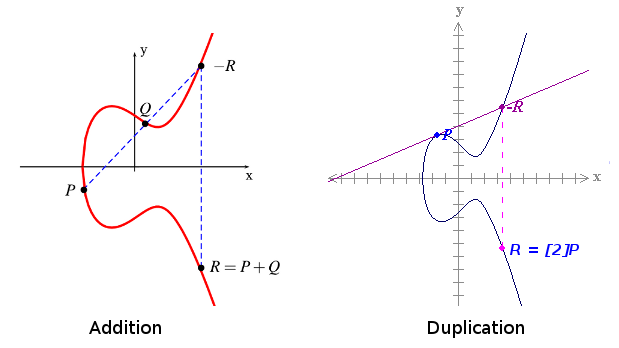
\includegraphics[scale=0.7]{images/ec}\\

\vspace{1cm}
Picture 1: ECDH schema\\
\end{center}

\vspace{1cm}
\subsubsection{Elliptic Curves Diffie Hellman key exchange}
The Diffie-Hellman key exchange (DH) is a key-agreement protocol used to generate a common secret between the two parts over an insecure channel; the computed secret is guaranteed to be the same for both and it's in the form of a byte array (in our case with length 32). From that secret then a deterministic key generation algorithm is able to extract a symmetric key usable for encryption/decryption. The Elliptic Curves DH (ECDH) works like this: every part computes a key pair over the same EC (we use the ones computed in the wizard), then both send their own public key to the other; now they multiply (for a proper definition on multiplication in a EC field) the public key of the other by their own private key: the result is the same due to the public/private EC keys mathematical properties as shown in the picture below.\\

\vspace{1cm}
\begin{center}
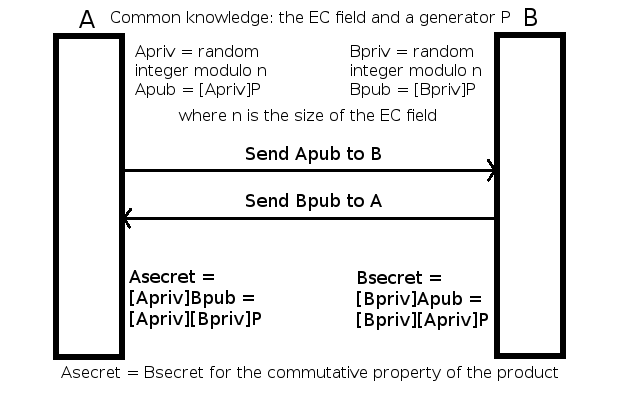
\includegraphics[scale=0.7]{images/ecdh}\\

\vspace{1cm}
Picture 1: ECDH schema\\
\end{center}

\vspace{1cm}
The problem with ECDH is the lack of authentication of the received public key: an active MITM could impersonate user A with user B and user B with user A by tricking them into believe his public key belongs to the other side while actually it's not true. This single point of failure is solved by embedding ECDH into SMP (see section 4.3.6).
\clearpage
\subsubsection{Elliptic Curves Digital Signature Algorithm}
Nowadays ECDSA is the best known algorithm for computing digital signature with a reasonable size, high performances and very high security: it's the EC variant of the DSS-DSA algorithm and it works like this: assumed the signer (sender) has a keypair based on EC (Apriv = s, Apub = [s]P), and the receiver knows Apub and trusts it, and both parts know the curve and its parameters (n = size of the group, P a generator of the group), then:
\linebreak
\begin{enumerate}
\item The signer chooses a random integer $r$ $mod$ $n$ such that $n > 0$ and $GCD(r,n) = 1$
\item The signer computes $[r]P = (x,y)$
\item If $x = 0$ goto step 1, else the signer stores $x$ as $k$
\item The signer computes $r^{-1}$ $mod$ $n$ and $e = SHA-1(m)$ where $m$ is the message to sign
\item The signer computes $z = r^{-1}(e + sk)$ $mod$ $n$
\item If $z = 0$ goto step 1, else the signature is made by $(k,z)$
\linebreak
\end{enumerate}
Verification:
\linebreak
\begin{enumerate}
\item The receiver checks whether $k$ and $z$ are $mod$ $n$ and positive not null integers, if not, the signature is not valid
\item The receiver computes $e = SHA-1(m)$ and $w = z^{-1}$ $mod$ $n$
\item The receiver computes $u_{1} = ew$ $mod$ $n$ and $u_{2} = kw$ $mod$ $n$
\item The receiver computes a point $X = [u_{1}]P + [u_{2}][s]P$ and stores it as $(x,y)$
\item If $X$ is the point at infinity or is not verified $x = k$ $mod$ $n$, the signature is not valid, otherwise is valid.
\end{enumerate}
\subsubsection{PBKDF2 with HMAC-SHA-256}
The Password Based Key Derivation Function \#2 is a deterministic key-derivation algorithm which generates a symmetric crypto key with a desired length by taking in input a password or a passphrase (in our case the secret from ECDH) and a salt (which makes possible to derivate different keys from the same password) and doing a certain number (4096 in our case) of application of a pseudorandom function (HMAC-SHA-256 in our case) to them in the so called "key stretching", which makes very hard the use of rainbow tables for cryptanalysis.
\subsubsection{AES-256-GCM}
\small{The Advanced Encryption Standard is the symmetric encryption standard algorithm (NIST FIPS-197) almost worldwide since 2001, and it's known for high performances and security against cryptanalysis; in the application we employed its version with a 256 bits key, which has a security margin comparable to RSA with a 15360 bits key. Actually, since it's used in Galois/Counter Mode (GCM), it does not encrypt directly the plaintext, but it's instead used together with a 12 bytes initialization vector IV (which doesn't need to be secret, but unpredictable for every encryption, so the best choice is to pick it up randomly) to generate a pseudorandom keystream, which is then XORed to the plaintext: basically the block cipher simulates a stream cipher (so no padding is needed for the plaintext, whose length, thus, does not need to be a multiple of 16 bytes, like in direct encryption, which is a good thing, considering the 140 bytes limit for Android messages) which simulates a One Time Pad (OTP), the only cipher perfectly secure. Obviously AES-GCM is not perfectly secure because, frist, soon or later, a new key will be equal to one used in the past (not so soon though), second, the key is shorter than the plaintext and, third, the keystream is only pseudorandom. In addition to this the GCM mode generates also a 16 bytes Message Authentication Code (MAC) which is prepended to the ciphertext in order to provide an additional integrity check. Before the decryption (which needs of course the same IV and the same key) the message integrity is verified and, if it's not the case, an exception is raised and the command session is aborted. In GCM mode it's also possible to attach to the ciphertext some non-encrypted data (called Additional Authenticated Data, AAD) which are used along with the ciphertext itself to produce the MAC; in our case this feature is useless, so no AAD.\\The three pictures below show the encryption and the decryption under GMC (P = plaintext, K = key, C = ciphertext, A = AAD, T = MAC) and the AES encryption/decryption used to generate the keystream.}\\

\vspace{1cm}
\begin{center}
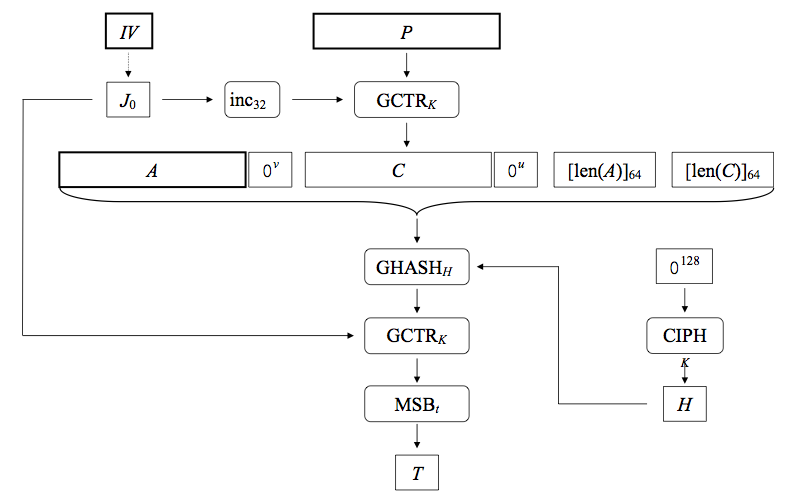
\includegraphics[scale=0.5]{images/aesgcmenc}\\

\vspace{1cm}
Picture 1: Encryption in GCM mode of operation\\
\clearpage
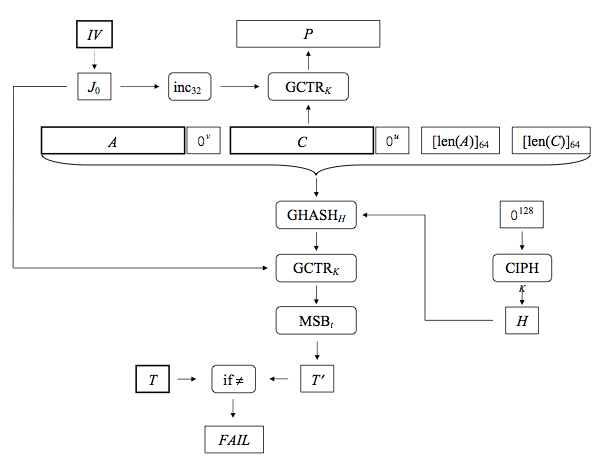
\includegraphics[scale=0.6]{images/aesgcmdec}\\

\vspace{0.5cm}
Picture 2: Decryption in GCM mode of operation\\

\vspace{2cm}
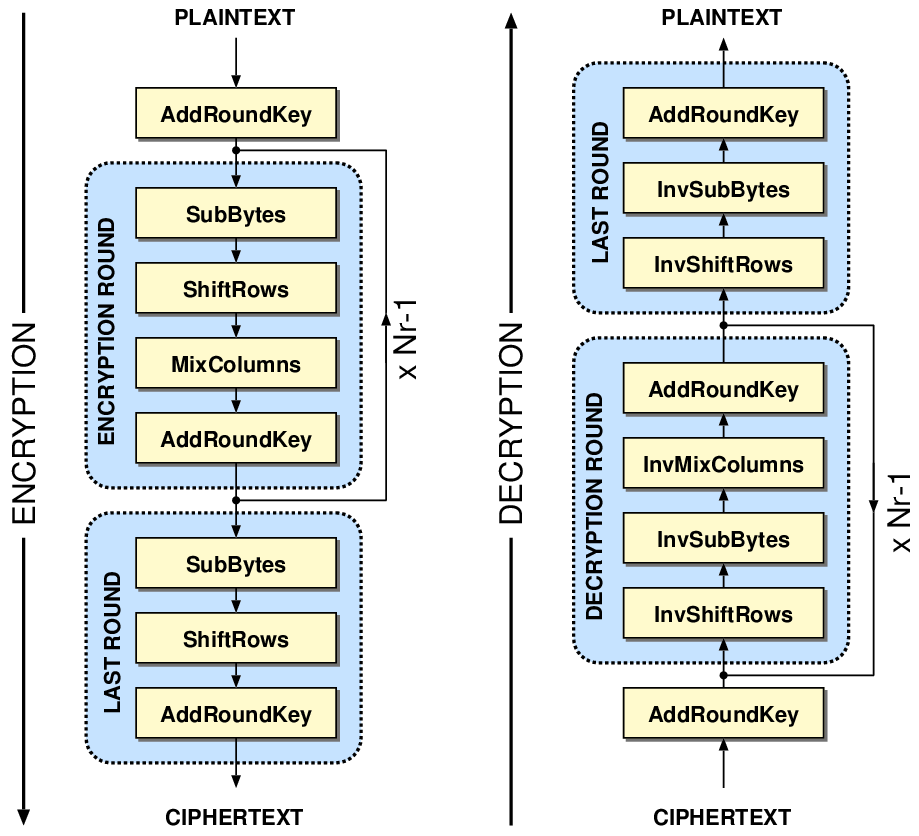
\includegraphics[scale=0.3]{images/aes}

\vspace{0.5cm}
Picture 3: Encryption/Decryption in AES\\
\end{center}
\clearpage
\subsubsection{Socialist Millionaire Protocol}
\paragraph{Public key request}
\paragraph{Public key sending}
\paragraph{Question sending}
\paragraph{Hash sending}
\paragraph{Ack and password salt sending}
\paragraph{Second half}
\paragraph{Error management}
\subsubsection{Command Protocol}
\paragraph{First message}
\paragraph{Second message}
\paragraph{Third message}
\paragraph{Fourth message}
\paragraph{Error management}
\paragraph{Timeout management}

\noindent
\Huge{\section{Testing}}
\subsection{Cryptography}
\subsection{Protocols}
\clearpage

\noindent
\Huge{\section{Installation and usage manual}}
\subsection{Installation}
\subsection{Usage}
\subsubsection{Initialization wizard}
\subsubsection{Change application settings}
\subsubsection{Send a command message}
\clearpage

\end{document}